%%%%%%%%%%%%%%%%%%%%%%%%%%%%%%%%%%%%%%%%%
% Wenneker Assignment
% LaTeX Template
% Version 2.0 (12/1/2019)
%
% This template originates from:
% http://www.LaTeXTemplates.com
%
% Authors:
% Vel (vel@LaTeXTemplates.com)
% Frits Wenneker
%
% License:
% CC BY-NC-SA 3.0 (http://creativecommons.org/licenses/by-nc-sa/3.0/)
% 
%%%%%%%%%%%%%%%%%%%%%%%%%%%%%%%%%%%%%%%%%

%----------------------------------------------------------------------------------------
% PACKAGES AND OTHER DOCUMENT CONFIGURATIONS
%----------------------------------------------------------------------------------------

\documentclass[11pt]{scrartcl} % Font size

%%%%%%%%%%%%%%%%%%%%%%%%%%%%%%%%%%%%%%%%%
% Wenneker Assignment
% Structure Specification File
% Version 2.0 (12/1/2019)
%
% This template originates from:
% http://www.LaTeXTemplates.com
%
% Authors:
% Vel (vel@LaTeXTemplates.com)
% Frits Wenneker
%
% License:
% CC BY-NC-SA 3.0 (http://creativecommons.org/licenses/by-nc-sa/3.0/)
% 
%%%%%%%%%%%%%%%%%%%%%%%%%%%%%%%%%%%%%%%%%

%----------------------------------------------------------------------------------------
%	PACKAGES AND OTHER DOCUMENT CONFIGURATIONS
%----------------------------------------------------------------------------------------

\usepackage{amsmath, amsfonts, amsthm} % Math packages

\usepackage{listings} % Code listings, with syntax highlighting

\usepackage[english]{babel} % English language hyphenation

\usepackage{graphicx} % Required for inserting images
\graphicspath{{Figures/}{./}} % Specifies where to look for included images (trailing slash required)

\usepackage{booktabs} % Required for better horizontal rules in tables

\numberwithin{equation}{section} % Number equations within sections (i.e. 1.1, 1.2, 2.1, 2.2 instead of 1, 2, 3, 4)
\numberwithin{figure}{section} % Number figures within sections (i.e. 1.1, 1.2, 2.1, 2.2 instead of 1, 2, 3, 4)
\numberwithin{table}{section} % Number tables within sections (i.e. 1.1, 1.2, 2.1, 2.2 instead of 1, 2, 3, 4)

\setlength\parindent{0pt} % Removes all indentation from paragraphs

\usepackage{enumitem} % Required for list customisation
\setlist{noitemsep} % No spacing between list items

%----------------------------------------------------------------------------------------
%	DOCUMENT MARGINS
%----------------------------------------------------------------------------------------

\usepackage{geometry} % Required for adjusting page dimensions and margins

\geometry{
	paper=a4paper, % Paper size, change to letterpaper for US letter size
	top=2.5cm, % Top margin
	bottom=3cm, % Bottom margin
	left=3cm, % Left margin
	right=3cm, % Right margin
	headheight=0.75cm, % Header height
	footskip=1.5cm, % Space from the bottom margin to the baseline of the footer
	headsep=0.75cm, % Space from the top margin to the baseline of the header
	%showframe, % Uncomment to show how the type block is set on the page
}

%----------------------------------------------------------------------------------------
%	FONTS
%----------------------------------------------------------------------------------------

\usepackage[utf8]{inputenc} % Required for inputting international characters
\usepackage[T1]{fontenc} % Use 8-bit encoding

\usepackage{fourier} % Use the Adobe Utopia font for the document

%----------------------------------------------------------------------------------------
%	SECTION TITLES
%----------------------------------------------------------------------------------------

\usepackage{sectsty} % Allows customising section commands

\sectionfont{\vspace{6pt}\centering\normalfont\scshape} % \section{} styling
\subsectionfont{\normalfont\bfseries} % \subsection{} styling
\subsubsectionfont{\normalfont\itshape} % \subsubsection{} styling
\paragraphfont{\normalfont\scshape} % \paragraph{} styling

%----------------------------------------------------------------------------------------
%	HEADERS AND FOOTERS
%----------------------------------------------------------------------------------------

\usepackage{scrlayer-scrpage} % Required for customising headers and footers

\ohead*{} % Right header
\ihead*{} % Left header
\chead*{} % Centre header

\ofoot*{} % Right footer
\ifoot*{} % Left footer
\cfoot*{\pagemark} % Centre footer
 % Include the file specifying the document structure and custom commands
\usepackage{hyperref} % Include the hyperref package for URLs
\usepackage[backend=bibtex,style=numeric]{biblatex}
\usepackage{csquotes}
\usepackage{algorithm}
\usepackage{algpseudocode}
\addbibresource{Bibliography.bib} % Specify the bibliography file (ensure this file exists and contains entries)


%----------------------------------------------------------------------------------------
% TITLE SECTION
%----------------------------------------------------------------------------------------

\title{	
	\normalfont\normalsize
	\textsc{University of Galway}\\ % Your university, school and/or department name(s)
	\vspace{25pt} % Whitespace
	\rule{\linewidth}{0.5pt}\\ % Thin top horizontal rule
	\vspace{20pt} % Whitespace
	{\huge  Project 1: Evolutionary Search (GAs)}\\ % The assignment title
	\vspace{12pt} % Whitespace
	\rule{\linewidth}{2pt}\\ % Thick bottom horizontal rule
	\vspace{12pt} % Whitespace
}

\author{\LARGE Cathal Lawlor} % Your name

\date{\normalsize\today} % Today's date (\today) or a custom date

\begin{document}

\maketitle % Print the title

\section{Github Repository}
Github repository with code available \href{https://github.com/Laan33/ai_project_1}{here}

\section{Implementation details \& design choices}

\subsection{Selection method}
I implemented and tried roulette wheel selection, tournament selection and the monte carlo selection methods.
I found tournament to be the most reliable, and easiest to implement in python, to actually get consistent, repeatable results (that actually worked).

As I'll elaborate on further in the potential improvements section \ref{Potential improvements}, I believe that tournament selection is the best choice for the travelling salesperson problem.
It is suited well for the TSP, as it maintains a good diversity in the population, and doesn't suffer from early convergence like roulette wheel selection can\cite{genetic_algorithm_afternoon}.

\subsection{Crossover methods}

I implemented both ordered crossover and partially mapped crossover. 

In partially mapped crossover (PMX)\cite{baeldung_pmx}, a random section of genes from one parent is copied to the child. The corresponding genes from the other parent are then mapped to avoid duplicates, ensuring each value appears exactly once. This method helps preserve relative positions within the crossover section.

In ordered crossover (OX)\cite{ordered_crossover_stackoverflow}, a random section of genes from one parent is copied to the child. The remaining positions are filled with genes from the other parent, in the order they appear, while skipping any duplicates. This ensures that the child inherits the relative ordering of cities from both parents.

I picked these two, as they both will work well for the travelling salesman problem, as they both preserve the order of the cities in the parents, which is crucial for TSP, by ensuring that good sequences are passed to the next generation. However, they differ in how they balance exploration and exploitation:

\begin{itemize}
    \item \textbf{PMX} supports more \textbf{exploitation} of the current solution by maintaining the relative positions of cities, which can result in faster convergence to a local optimum. This method tends to produce more similar offspring to the parents, making it more reliable but potentially limiting the diversity in the population, especially in the early stages of the algorithm.
    
    \item \textbf{OX}, on the other hand, fosters greater \textbf{exploration} by allowing more randomness in the order of cities. While this can lead to larger variations in offspring, it also means the algorithm has a better chance of avoiding local optima and exploring a broader solution space. This approach is particularly useful early in the evolution process when diversity in the population is needed to avoid premature convergence.
\end{itemize}

I chose these, as while PMX is more likely to produce a better child, OX can provide a more diverse population, which can be useful in the early stages of the algorithm and it will be interesting to see how they compare.

\subsection{Mutation methods}

I implemented both swap mutation and inversion mutation.

In swap mutation, two random cities in the tour are selected, and their positions are exchanged. This introduces small, random changes while preserving the tour length.

In inversion mutation, a random subsection of the tour is selected, and the order of cities within that section is reversed. This helps the algorithm explore new solutions while maintaining most of the existing tour structure.

I chose these because they introduce different types of variations in the population. Swap mutation makes small changes that can help fine-tune solutions, while inversion mutation can make larger changes that help the algorithm escape local optima. 
I wanted to see, when compairing both methods, the differences in the makeup of the algorithm.

\subsection{Termination condition}
I implemented a max number of generations to run, but I also added a clause, that if the algorithm hasn't improved by more than 0.25\% in the last 60 generations, it will terminate early.

This is because, genetic algorithms can get stuck in local optima, or just simply converge.

\begin{figure}[h!]
	\centering
	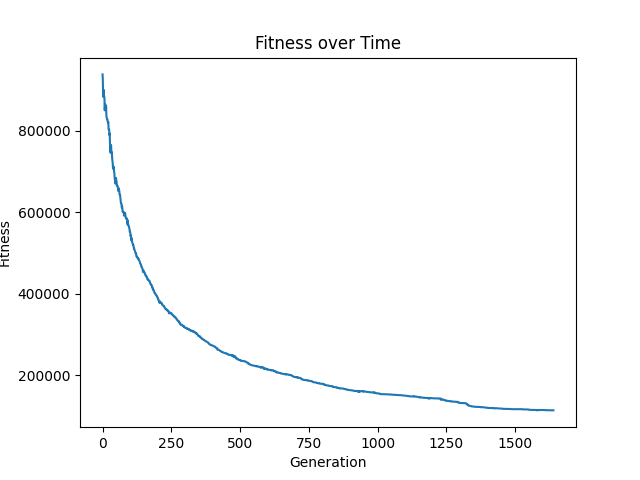
\includegraphics[width=0.8\linewidth]{convergence_example_.png}
	\caption{Example of convergence over generations}
	\label{fig:convergence_example}
\end{figure}

The above figure shows an example of convergence over generations, and how the algorithm will cut it off early, if it hasn't improved significantly (where this was to run to 2000 generations, it stopped at ~1620)
%------------------------------------------------

\section{Experimentation results \& analysis}

\subsection{Experimentation setup}
To evaluate the performance of the genetic algorithm (GA) for the travelling salesperson problem (TSP), I ran experiments on three different datasets: berlin52, kroA100, and pr1002.

I implemented grid search to fine-tune hyperparameters, including population size, crossover rate, mutation rate, and tournament size. The algorithm was run for each combination of hyperparameters.

I also implemented a gridsearch method for the crossover and mutation methods, to see which would work best for the TSP.

\subsection{Method testing results}
\begin{table}[h!]
	\centering
	\begin{tabular}{|c|c|c|c|c|c|c|c|}
	\hline
	\textbf{Best Fitness} & \textbf{Time (s)} & \textbf{Iterations} & \textbf{Mutation Method} & \textbf{Crossover Method} \\ \hline
	9709.39 & 3.373 & 496 & swap\_mutation & ordered\_crossover \\ \hline
	9974.86 & 2.492 & 400 & swap\_mutation & partially\_mapped\_crossover \\ \hline
	8962.86 & 2.63 & 400 & inversion\_mutation & ordered\_crossover \\ \hline
	\textbf{8124.54} & \textbf{2.391} & \textbf{400} & \textbf{inversion\_mutation} & \textbf{partially\_mapped\_crossover} \\ \hline
	\end{tabular}
	\caption{Comparison of different GA configurations}
	\label{tab:method_testing_results}
\end{table}

For all of the above tests, the following parameters were used:
\begin{table}[h!]
	\centering
	\begin{tabular}{|c|c|c|}
	\hline
	\textbf{Population Size} & \textbf{Mutation Rate} & \textbf{Crossover Rate} \\ \hline
	200 & 0.15 & 0.87 \\ \hline
	\end{tabular}
	\caption{GA Parameters}
	\label{tab:params}
\end{table}

\subsubsection{Best crossover method}
In my quick experiment on berlin52, PMX achieved the best score alongside inversion mutation, but when PMX and OX were paired with swap mutation, OX had a better fitness. 
This was still far off the mark of using inversion mutation, but it might be that ordered crossover is better when it's with swap mutation, 
as it can provide a more diverse population (when swap mutation may not be enough to provide that diversity).

It could also be down to the parameters used, as these are close to the best parameters, which were found using inversion mutation and PMX.

\subsubsection{Best mutation method}
Inversion mutation proved to lead to better overall solutions compared to swap mutation. Inversion mutation may have allowed the algorithm to escape local optima more effectively, where swap mutation may have been too conservative and better for fine tuning.

\subsubsection{Best parameters}
Through grid search, I identified the following optimal hyperparameters for the TSP datasets:

\begin{table}[h!]
	\centering
	\begin{tabular}{|c|c|c|c|}
	\hline
	\textbf{Dataset} & \textbf{Population Size} & \textbf{Crossover Rate} & \textbf{Mutation Rate} \\ \hline
	\textbf{berlin52} & 470 & 0.9 & 0.12 (inversion mutation used) \\ \hline
	\textbf{kroA100} & 470 & 0.71 & 0.2 (inversion mutation used) \\ \hline
	\end{tabular}
	\caption{Optimal hyperparameters for TSP datasets}
	\label{tab:optimal_params}
\end{table}

Notably for me, both datasets favored a relatively large population size, which will have helped maintain a diverse population and avoid premature convergence (avoiding getting stuck in local optima). 

For berlin52, the higher crossover rate might suggest that more aggressive exploration was beneficial as it's a smaller problem instance, whereas the kroA100 dataset required a more balanced approach with a higher mutation rate to escape local optima.


\section{Comparison with known optimal solutions}
\label{Comparison with known optimal solutions}

Comparing to the optimal solutions from Heidelberg university \cite{heidelberg_university_best_known}, my algorithm achieved reasonably good results on the smaller datasets.

It really struggled with the larger Pr1002 dataset, which I expected for my basic GA. 
I was bound by both time and computing power, so I couldn't run the algorithm for long enough to get a good solution, with a much higher population size, allowing more generations before convergence.

\begin{table}[h!]
\centering
\begin{tabular}{|c|c|c|c|}
\hline
\textbf{Dataset} & \textbf{My Algorithm} & \textbf{Optimal Solution} & \textbf{Difference} \\ \hline
\textbf{berlin52} & 7,700.2 & 7,542 & 2.1\% \\ \hline
\textbf{kroA100} & 23,171.6 & 21,282 & 8.88\% \\ \hline
\textbf{pr1002} & 1,318,922.4 & 259,045 & 409\% \\ \hline
\end{tabular}
\caption{Comparison of algorithms with known optimal solutions}
\label{tab:comparison}
\end{table}

The differnece for pr1002 dataset is very large, but I think it will come down drastically with a larger population size, and more generations.

\section{Potential improvements}
\label{Potential improvements}
One easy, improvment I believe for my algorithm would be to employ elitism.
I implemented it in a early version of the program. I chose not to implement it, as I wanted to see how the various methods for crossover and mutation would handle the problem alone, without the help of elitism.
It would probably extract a small bit more performance out, especially for the bigger datasets, less so in the Berlin dataset.

I believe that tournament selection is a good choice, being the sweet spot for a genetic algorithm solving TSP. It's fast, simple, and maintains a good diversity and doesn't suffer with early convergence like roulette wheel selection can\cite{genetic_algorithm_afternoon}.
I also tried monte carlo selection, but I do not believe it works for the travelling salesperson problem.

Another, is to run the same parameters multiple times on differening starting populations, and averaging the results. This would give a more accurate representation of the algorithm's performance, as the starting population can have a big impact on the final result. e.g. it may get stuck in a local optima, or converge too early.
Also related to this, is to allow the algorithm to do hyperparameter tuning on the fly (e.g. using adaptive mutation or crossover rates based on fitness), as it's running. This would allow the algorithm to adjust to the problem, and the population, as it's running, and not just at the start.

For the bigger pr1002 dataset, I think given more time and resources would help improve the results on the large pr1002 dataset. 
Mainly, this would allow me to up the population size by a lot, which then allows it to run for a lot more generations without converging too early, allowing more exploraiton of the solution space.

There is other improvements, such as a hybrid approach of a local search algorithm, e.g. 2-opt, to improve the final solution once the genetic algorithm has converged. This would help fine-tune the solution, and get a better result.
\section{Conclusions}

\printbibliography
\end{document}
